\documentclass{beamer}\usepackage[]{graphicx}\usepackage[]{color}
%% maxwidth is the original width if it is less than linewidth
%% otherwise use linewidth (to make sure the graphics do not exceed the margin)
\makeatletter
\def\maxwidth{ %
  \ifdim\Gin@nat@width>\linewidth
    \linewidth
  \else
    \Gin@nat@width
  \fi
}
\makeatother

\definecolor{fgcolor}{rgb}{1, 0.894, 0.769}
\newcommand{\hlnum}[1]{\textcolor[rgb]{0.824,0.412,0.118}{#1}}%
\newcommand{\hlstr}[1]{\textcolor[rgb]{1,0.894,0.71}{#1}}%
\newcommand{\hlcom}[1]{\textcolor[rgb]{0.824,0.706,0.549}{#1}}%
\newcommand{\hlopt}[1]{\textcolor[rgb]{1,0.894,0.769}{#1}}%
\newcommand{\hlstd}[1]{\textcolor[rgb]{1,0.894,0.769}{#1}}%
\newcommand{\hlkwa}[1]{\textcolor[rgb]{0.941,0.902,0.549}{#1}}%
\newcommand{\hlkwb}[1]{\textcolor[rgb]{0.804,0.776,0.451}{#1}}%
\newcommand{\hlkwc}[1]{\textcolor[rgb]{0.78,0.941,0.545}{#1}}%
\newcommand{\hlkwd}[1]{\textcolor[rgb]{1,0.78,0.769}{#1}}%
\let\hlipl\hlkwb

\usepackage{framed}
\makeatletter
\newenvironment{kframe}{%
 \def\at@end@of@kframe{}%
 \ifinner\ifhmode%
  \def\at@end@of@kframe{\end{minipage}}%
  \begin{minipage}{\columnwidth}%
 \fi\fi%
 \def\FrameCommand##1{\hskip\@totalleftmargin \hskip-\fboxsep
 \colorbox{shadecolor}{##1}\hskip-\fboxsep
     % There is no \\@totalrightmargin, so:
     \hskip-\linewidth \hskip-\@totalleftmargin \hskip\columnwidth}%
 \MakeFramed {\advance\hsize-\width
   \@totalleftmargin\z@ \linewidth\hsize
   \@setminipage}}%
 {\par\unskip\endMakeFramed%
 \at@end@of@kframe}
\makeatother

\definecolor{shadecolor}{rgb}{.97, .97, .97}
\definecolor{messagecolor}{rgb}{0, 0, 0}
\definecolor{warningcolor}{rgb}{1, 0, 1}
\definecolor{errorcolor}{rgb}{1, 0, 0}
\newenvironment{knitrout}{}{} % an empty environment to be redefined in TeX

\usepackage{alltt}
\usepackage{../371g-slides}
\title{Decision Trees - Part 1}
\subtitle{Lecture 20}
\author{STA 371G}
\IfFileExists{upquote.sty}{\usepackage{upquote}}{}
\begin{document}
  
  

  \frame{\maketitle}

  % Show outline at beginning of each section
  \AtBeginSection[]{ 
    \begin{frame}<beamer>
      \tableofcontents[currentsection]
    \end{frame}
  }

  %%%%%%% Slides start here %%%%%%%

  \begin{darkframes}
    
    %{slide 1}
    \begin{frame}{Making Better Decisions}
      \fontsize{10}{10}\selectfont
      \begin{center}
        
\includegraphics[width=2in]{DecisionAnalysis.png} \\
      \end{center}
        \textit{Decision making is the only way that individuals can purposely
        exercise any control over thier lives, careers, or their surroundings.}
        \text{- Ralph Keeney, Making Better Decision Makers, Decision Analysis, vol. 1}
        No:4, 2004
      
      \lc %{How do you make important decisions?}
    \end{frame}


    %{slide 2}
    \begin{frame}[fragile]{Decision Analysis}
    \fontsize{10}{10}\selectfont
      \begin{itemize}[<+->]
        \item A framework for analyszing decision problems that involve uncertainty
        \item Decision trees: a powerful graphical tool that guides that analysis
        \item Smaller analyses can be done using pen and paper
        \item Larger ones require software 
        \end{itemize} 
    \end{frame}


    %{slide 3}
    \begin{frame}[fragile]{Topics to Cover}
    \fontsize{10}{10}\selectfont
          \begin{itemize}[<+->]
            \item Criteria for choosing among alternative decisions
            \item How probabilities are used in the decision-making process
            \item How early decisions affect decisions make later
            \item How a decision maker can quantify the value of information
            \item How attitudes toward risk and uncertainty can affect the analysis
          \end{itemize}

    \end{frame}


    %{slide 4}
    \begin{frame}[fragile]{Elements of a Decision Analysis}
      \fontsize{10}{10}\selectfont  
      \text{Although decision making under uncertainty occurs in a wide variety of}
      \text{contexts, all problems have three common elements:}

        \begin{itemize}[<+->]
            \item The decisions available to the decision maker
            \item The possible outcomes and the probabilities of these outcomes
            \item A value model that provides values (in monetary units usually) for the various outcomes
        \end{itemize}

      \text{Once these elements are defined, the decision maker can find an}
      \text{optimal decision.}

    \end{frame}


    %{slide #5}
    \begin{frame}[fragile]{Payoff Tables}
      \fontsize{10}{10}\selectfont  
      \text{A payoff table lists the payoff for each decision outcome pair}
      \begin{itemize}
            \item Positive values are gains and negative values are losses
        \end{itemize}
        \begin{center}
          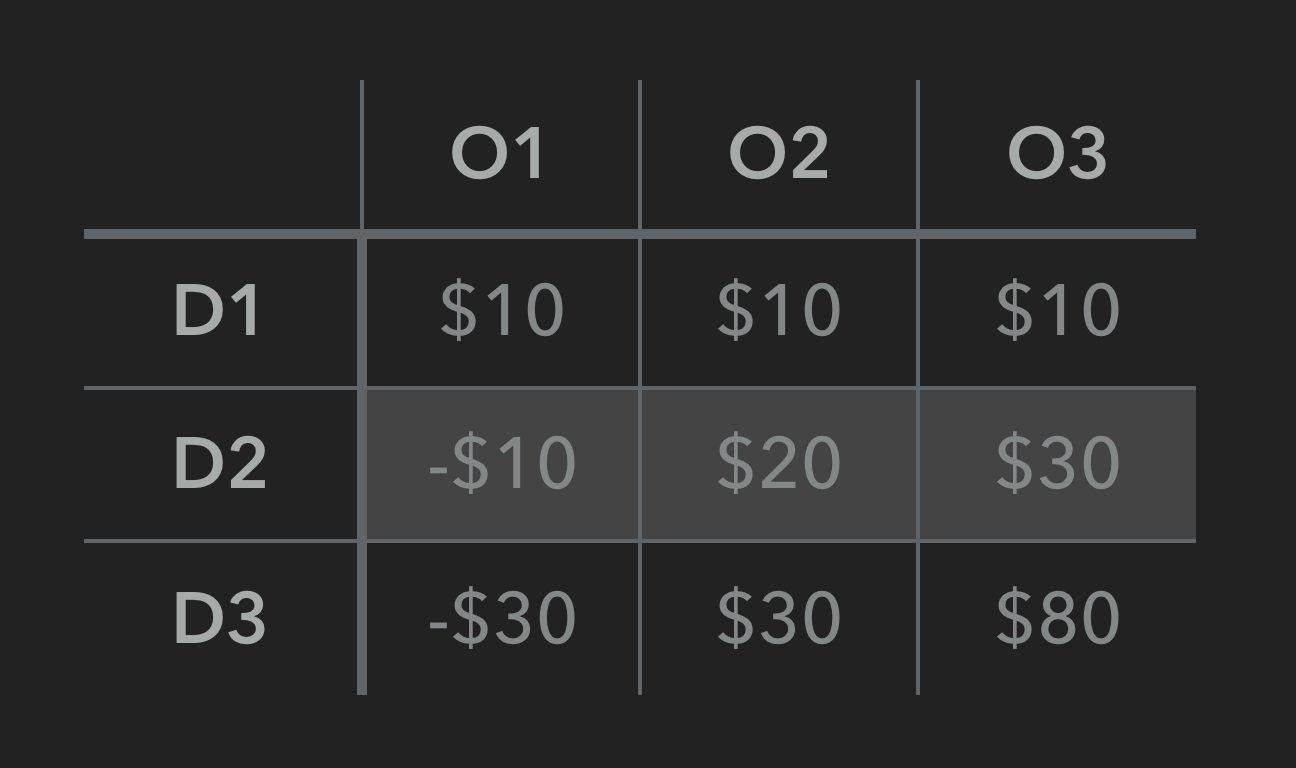
\includegraphics[width=3in]{PayoffTable} 
        \end{center}
        \begin{itemize}
            \item This table shows three possible decisions (D1, D2, and D3) and three
            possible outcomes (O1, O2, and O3) for each.
            \item Which decision do you prefer?
        \end{itemize}

      \lc %{Which decision do you prefer?}
    \end{frame}


    %{slide #6}
    \begin{frame}[fragile]{Payoff Tables}
      \fontsize{10}{10}\selectfont  
      \text{But we need probabilities for the outcomes to make a good decision}
      \begin{center}
        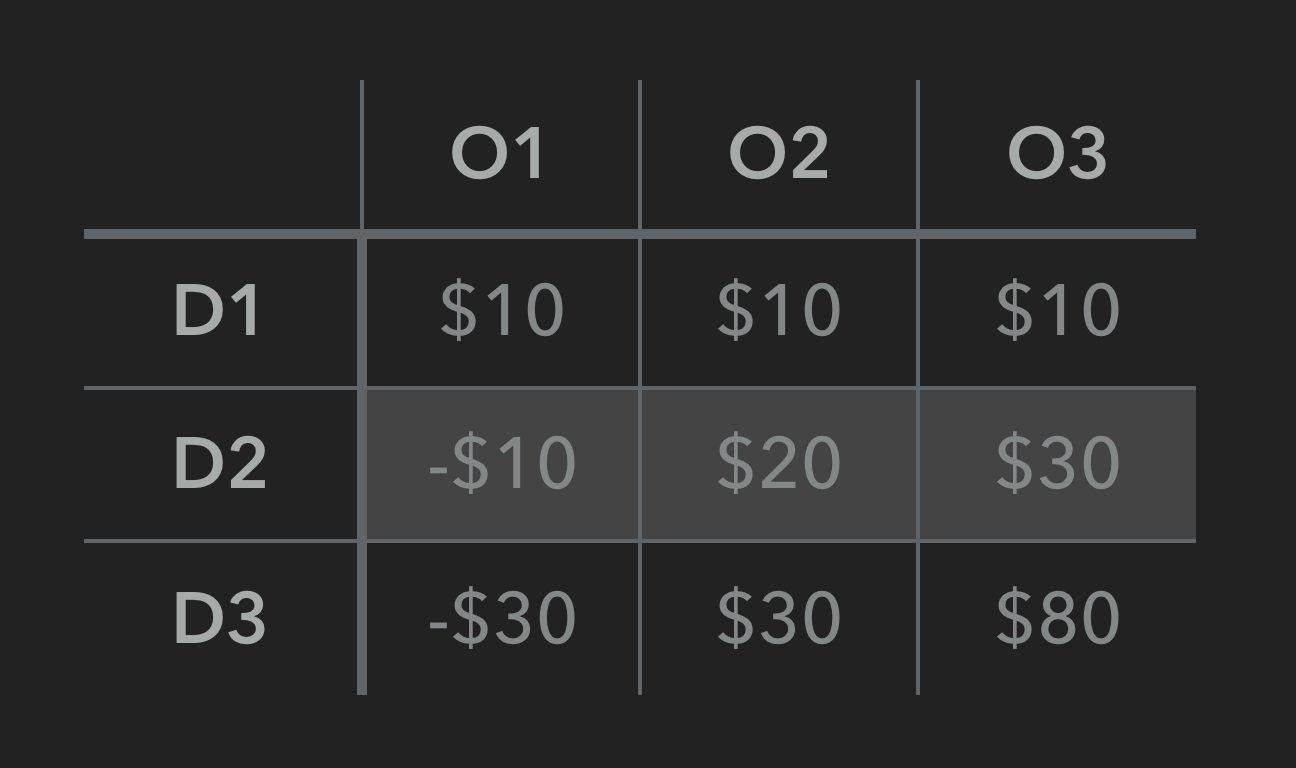
\includegraphics[width=3in]{PayoffTable} 
      \end{center}
        \begin{itemize}
            \item Probabilities: P(O1) = 0.3, P(O2) = 0.5, P(O3) = 0.2
            \item Now which decision do you prefer?
        \end{itemize}

    \end{frame}


    %{slide 7}
    \begin{frame}[fragile]{Expected Value - Remember this?}
      \fontsize{10}{10}\selectfont  
         \begin{itemize}
            \item EV is a weighted average of the possible payoffs for the decision,
            weighted by the probabilities of the outcomes
            \item D1: EV = 10
            \item D2: EV = -10(0.3) + 20(0.5) - 30(0.2) = 13 
            \item D3: EV = ?
        \end{itemize}    

      \lc %{What is EV of D3?}
    \end{frame}


    %{slide 8}
    \begin{frame}[fragile]{Decision Trees}
      \fontsize{10}{10}\selectfont 
          \begin{itemize}
            \item Time proceeds from left to right.
            \item Branches leading out of a decision node represent the possible decisions
            \item Probabilities are listed on probability branches. The probabilities are conditional on the events that have already been observed.
            \item Monetary values are shown to the right of the end nodes.
            \item EVs are calculated through a ``rolling-back'' process.
          \end{itemize}  
    \end{frame}


    %{slide 9}
    \begin{frame}[fragile]{Decision Tree For Our Simple Example}
      \fontsize{10}{10}\selectfont 
      \begin{center}
      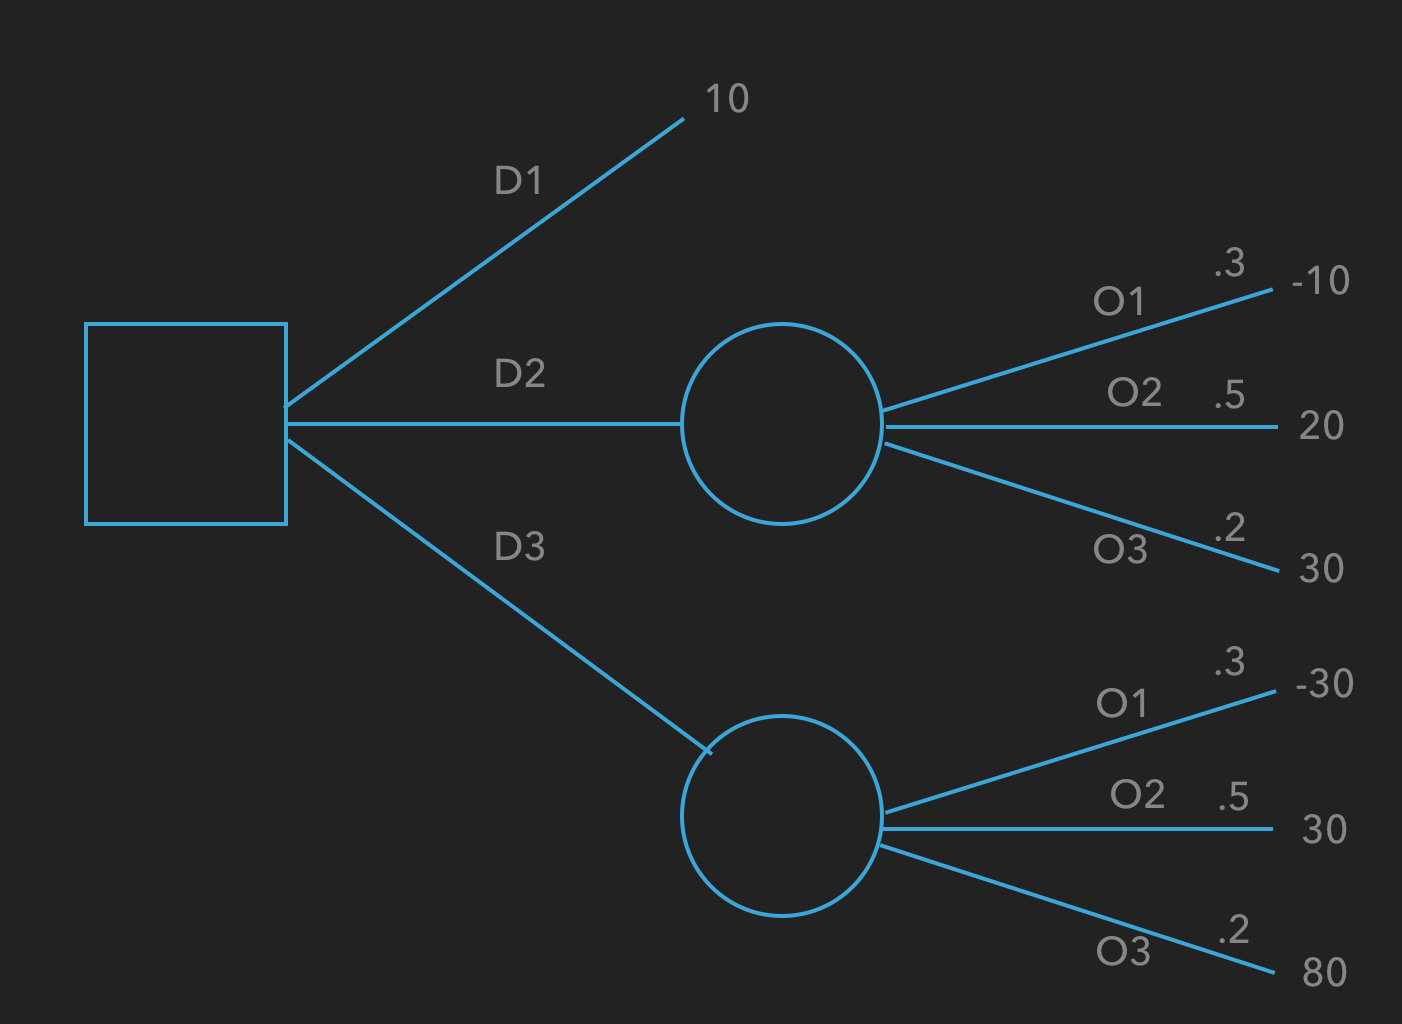
\includegraphics[width=3.5in]{DecisionTree} 
      \end{center}
    \end{frame}     


   %{slide 10}
    \begin{frame}[fragile]{Rollback Procedure}
      \fontsize{10}{10}\selectfont  
      \text{Calculate the expected value at each probability node}
      \begin{center}
      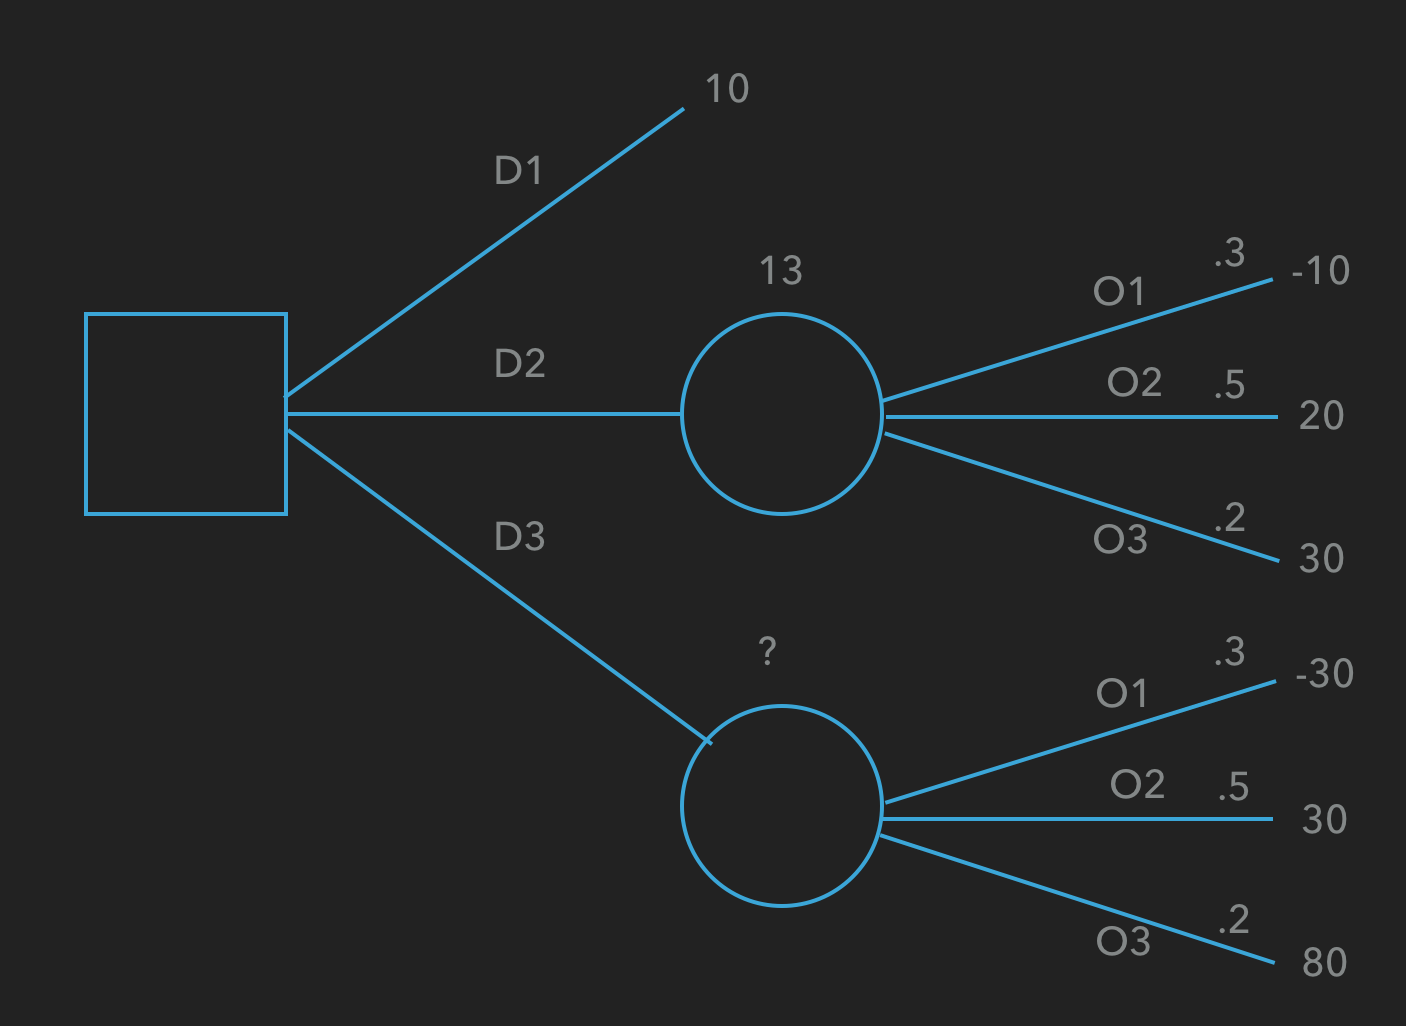
\includegraphics[width=3.5in]{RollingBack} 
      \end{center}

      \text{EV = .3(-10) + .5(20) + .2(30) = 13}

      \lc %{Calculate the node EV}
    \end{frame}

    %{slide 11}
    \begin{frame}[fragile]{Rollback Procedure}
      \fontsize{10}{10}\selectfont  
      \text{Calculate the maximum at each decision node}
      \begin{center}
      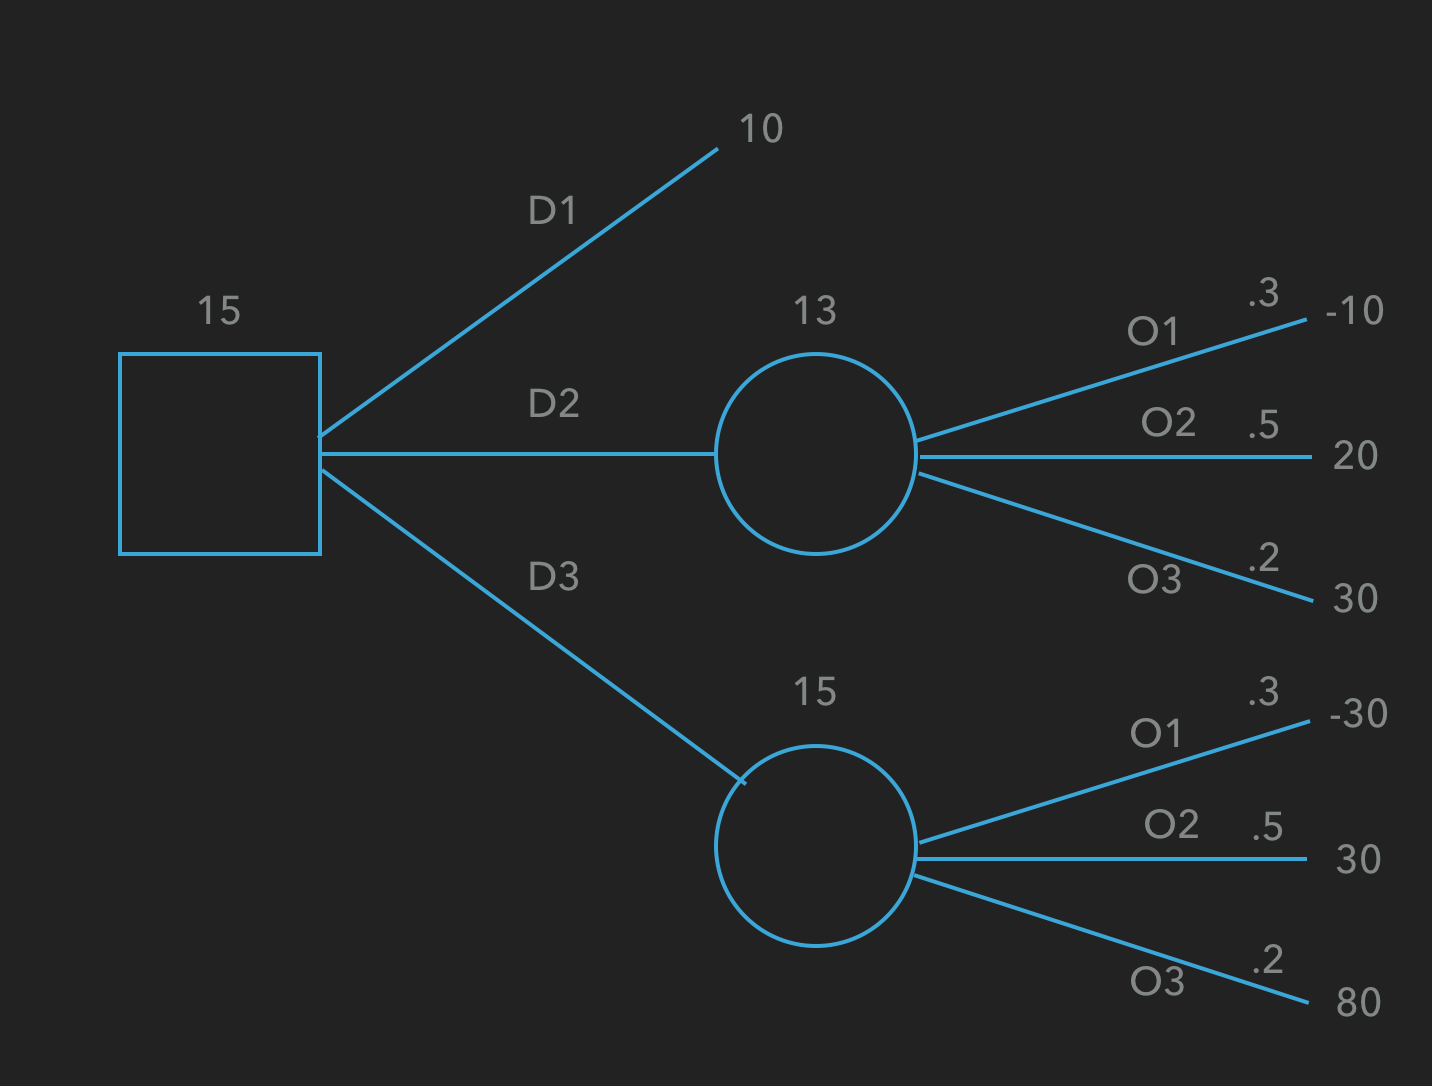
\includegraphics[width=3.5in]{FinalTree} 
      \end{center}

      \text{22 is the maximum out of of 10, 13, and 22}

    \end{frame}


    %{slide 12}
    \begin{frame}[fragile]{Sally Ann Soles' Shoe Factory}
     \fontsize{10}{10}\selectfont  
     \text{Sally Ann Soles manages a sucessful shoe factory. She is wondering } 
     \text{whether to expand her factory this year. The cost of the expansion is 1.5M USD} 
     \text{is 1.5M USD.} 

     \text{If she does nothing and the economy stays good, she expects to earn 3M in}
     \text{revenue, but if the economy is bad, she expects only 1M.} 
     \text{If she expands the factory, she expects to earn 6M if the economy is}
     \text{good and 2M if it is bad.} 

     \text{She also assumes that there is a 40 percent chance of a good economy and}
     \text{a 60 percent chance of a bad economy.} 

     \text{Should she expand?} 
    \end{frame}


    %{slide 13}
    \begin{frame}[fragile]{Shoe Factory Expansion Decision Tree}
    \fontsize{10}{10}\selectfont  
      \begin{center}
        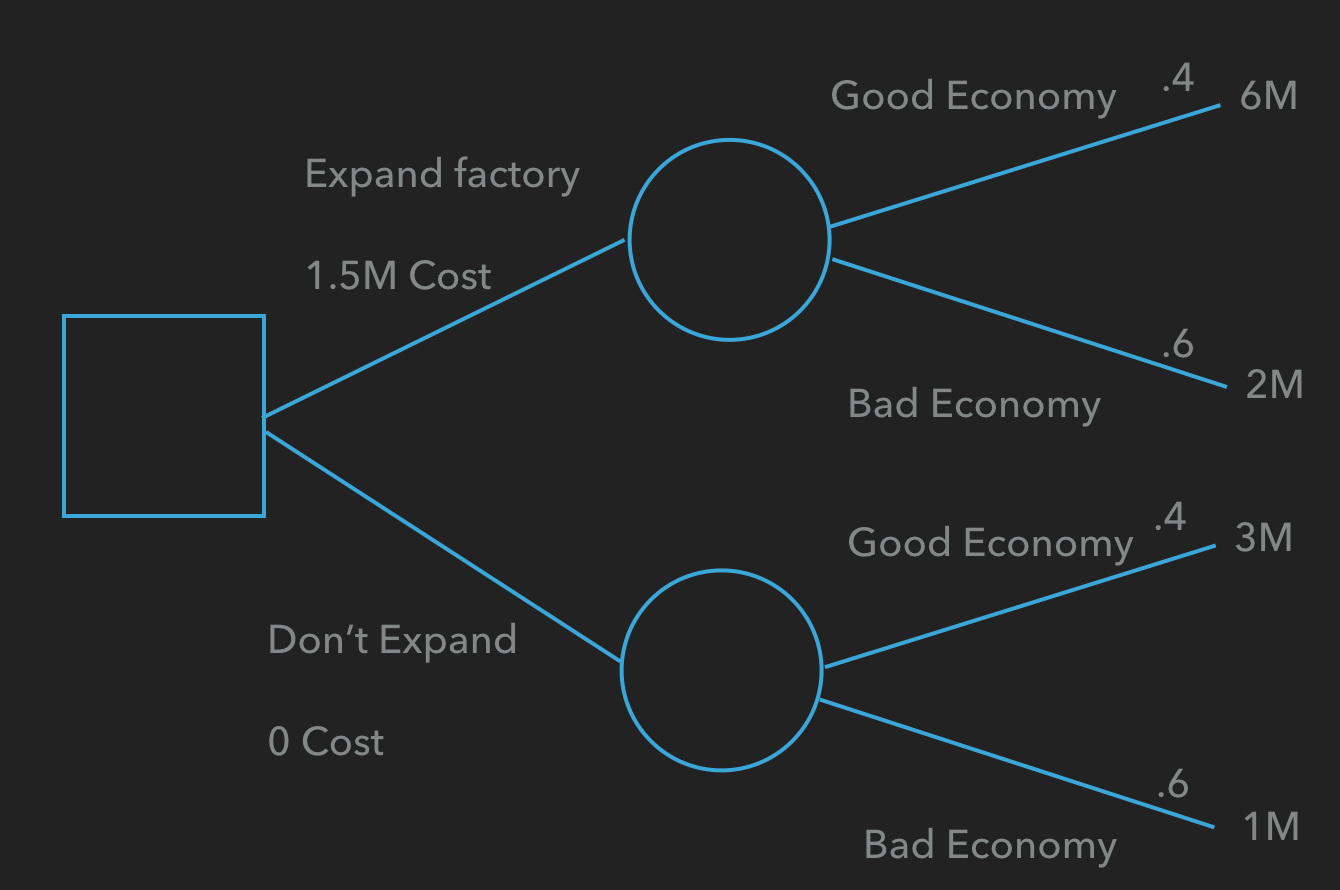
\includegraphics[width=3.5in]{ExpandFactory} \\
      \end{center}
    \text{EV(Expand) = (.4(6) + .6(2)) - 1.5 = 2.1M}
    \text{EV(No Expand) = (.4(3) + .6(1)) = 1.8M, }
    \text{2.1M > 1.8M, so she should expand!}
    \end{frame}


    %{slide 14}
    \begin{frame}[fragile]{Shoe Factory Expansion Decision Tree With An Option}
     \fontsize{10}{10}\selectfont  
     \text{A few days later, she was told that if she expands, she can opt to either} 
     \text{(a) expand the factory further, which costs 1.5M and will yield an extra} 
     \text{2M in profit if the economy is good, but 1M if it is bad,}
     \text{(b) abandon the project and sell the equipment she original bought for 1.3M,}
     \text{or (c) do nothing.} 


     \text{How has the decision changed?}
     \text{What is the value of this option before the state of the economy is known?}  
     \text{Intuitively, it might increase the value of the initial expansion.}
    \end{frame}

    %{slide 15}
    \begin{frame}[fragile]{A Sequential Decision}
      \begin{center}
        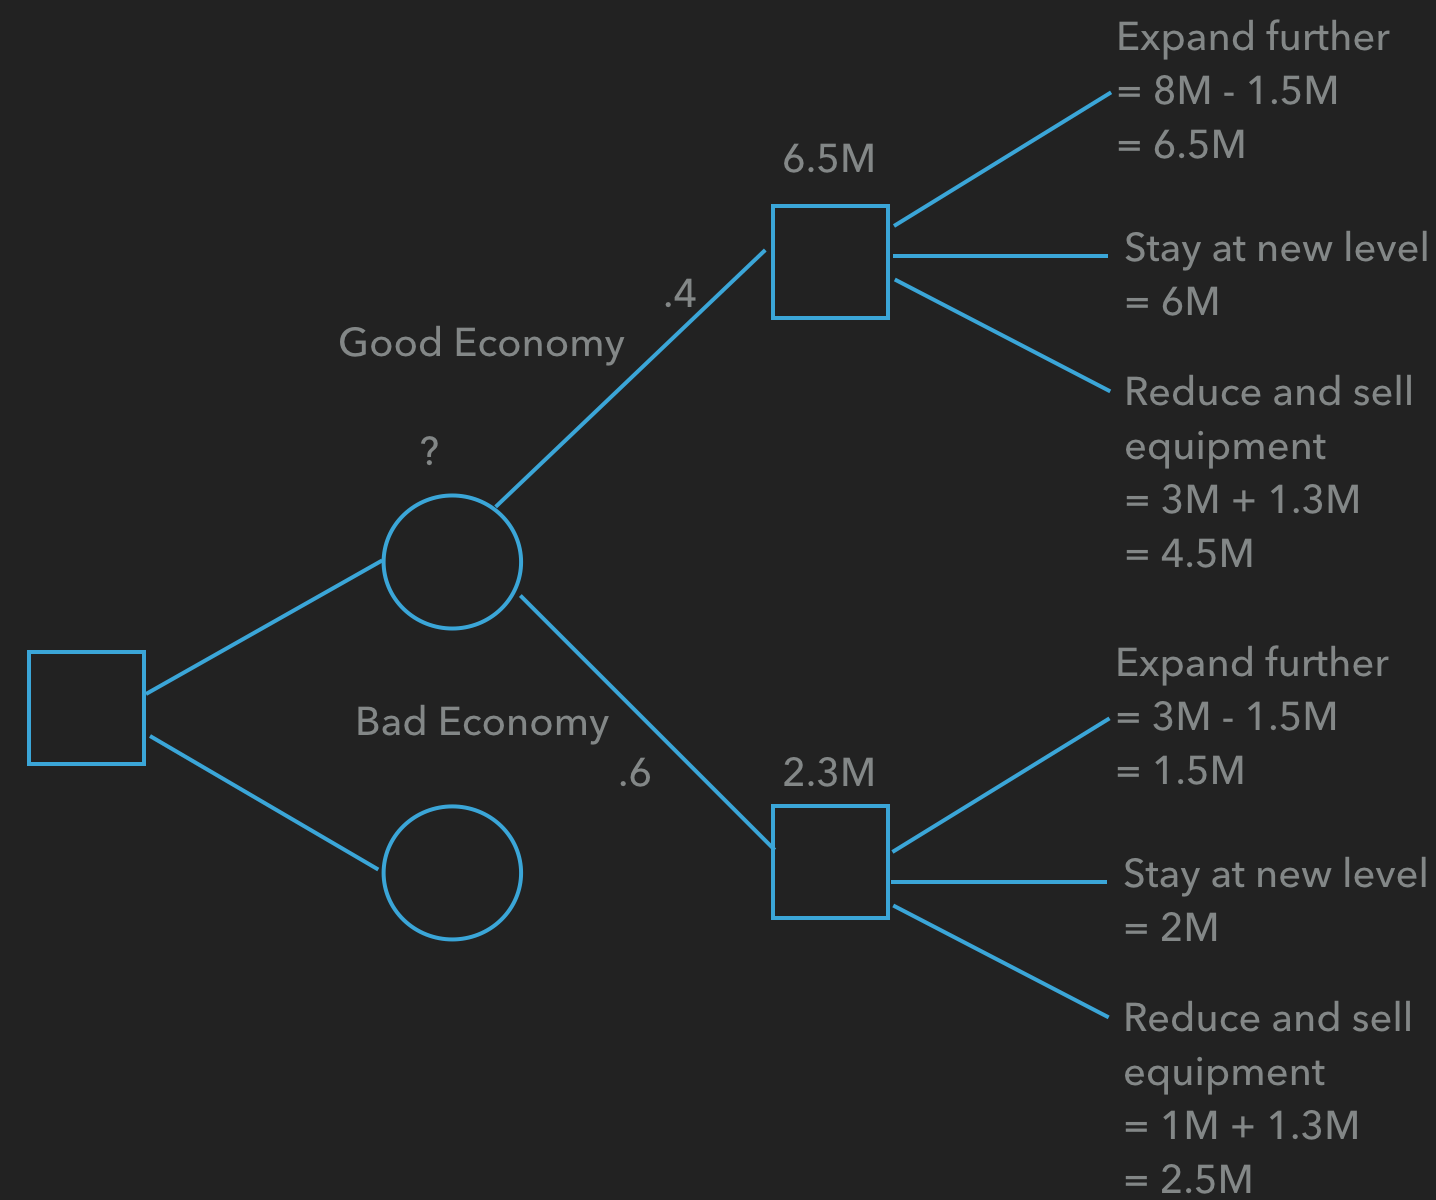
\includegraphics[width=3.5in]{SequentialDecision} \\
      \end{center}

    \lc %{Calculate the new Expansion EV} 
    \end{frame}


    %{slide 16}
    \begin{frame}[fragile]{What Is The Second Expansion Option's Value?}
      \begin{center}
        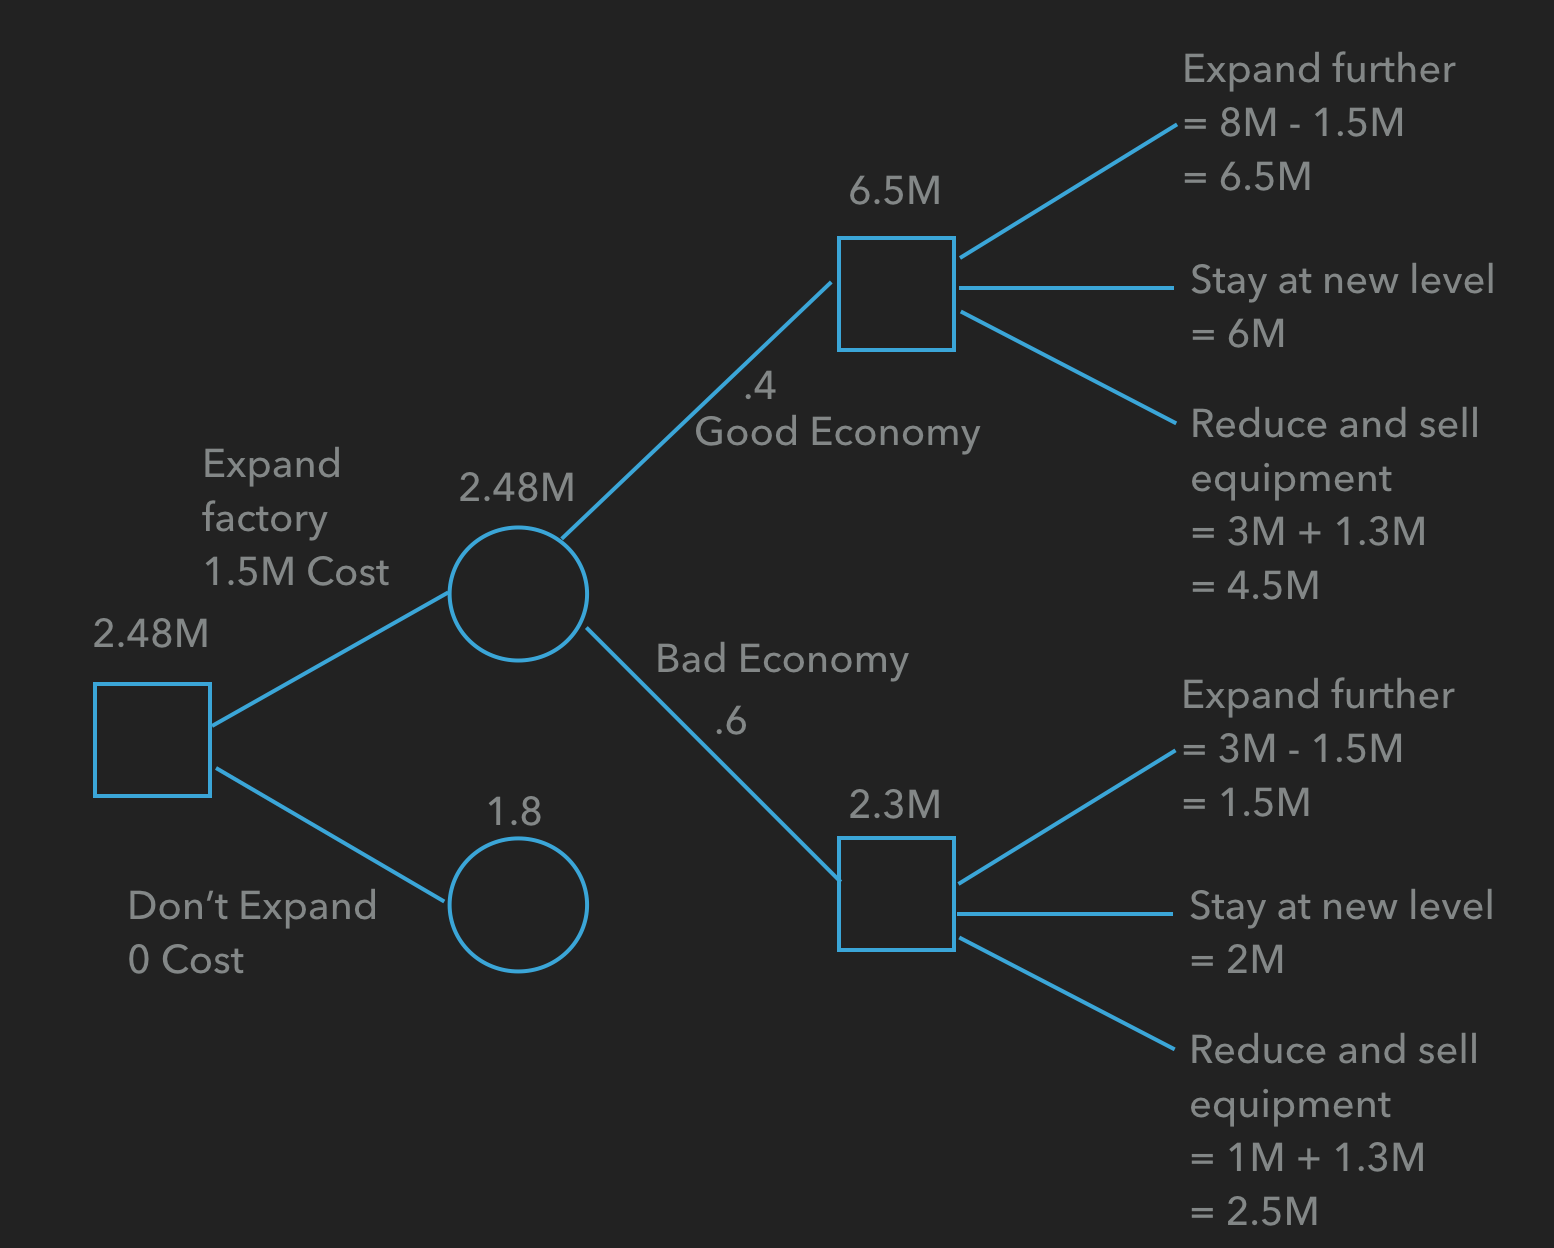
\includegraphics[width=3.5in]{FinalOption} \\
      \end{center}
    \end{frame}


    %{slide 17}
    \begin{frame}[fragile]{EV of the Project}
        \text{The EV of Expanding is now [.4(6.5) + .6(2.3)] - 1.5M = 2.48M}
        \text{Therefore the value of the option is:}
        \text{       new EV - old EV = 2.48M - 2.1M = 380,000 USD} 
    \end{frame}


   %{slide 18}
    \begin{frame}[fragile]{Does This Look Familiar?}
    \fontsize{10}{10}\selectfont  
       \text{This method of valuing real optionw is used by corpotate strategists,}
       \text{management consultants, and bankers. A further refinement is to take}
       \text{time value of money into account and present value the cashflows.}
  

    \end{frame}


    %{slide 19}
    \begin{frame}{More on Valuing Information Next Time...}
      \fontsize{10}{10}\selectfont

      \begin{itemize}
        \item Don't forget to do your Time Series homework!
        \item The TAs are still working on grading the test.
      \end{itemize}https://www.yahoo.com/news/analysis-trump-weight-worlds-problems-220503380.html
      
    \end{frame}

  \end{darkframes}
\end{document}
